\chapter{Higgs Searches \label{chapter3_analysis}}

\section{Higgs Discovery}
The experimental verfication of the existance of a Higgs boson and therefore the Higgs mechanism was found by
the two collaborations \CMS and \ATLAS in July 2012. The observation was found with a significance of $5.0\sigma$ ($5.9\sigma$)
at a Higgs boson mass of approximately $m_H=125$ GeV by \CMS (\ATLAS). It was necessary to combine different decay channel to
achieve the observation with the measured \LHC data of Run 1. Outstanding are the two golden channels $\PH \rightarrow \PZ \PZ \rightarrow 4\Plepton$ and
$\PH \rightarrow \Pgamma \Pgamma$, which profit from a high mass resolution and controllable backgrounds. Figure~\ref{figure_higgs_discovery_cms} shows the
discovery plots of both channel of the CMS collaboration.

\begin{figure}[h]
\includegraphics[width=0.48\textwidth]{../plots/HiggsGG_discovery.pdf}
\hfill
\includegraphics[width=0.48\textwidth]{../plots/HiggsZZ_discovery.pdf}
\caption[Higgs boson discovery CMS.]{Higgs boson discoveries in the two golden channels $\PH \rightarrow \Pgamma \Pgamma$ (left) and $\PH \rightarrow \PZ \PZ \rightarrow 4\Plepton$ (right) by \CMS~\cite{HiggsDiscovery_CMS}.}
\label{figure_higgs_discovery_cms}
\end{figure}

Both discovery plots cleary show an excess in the invariant mass distribution at around $m_H=125$ GeV. The left figure
shows the invariant mass of two photons in a range between $100$ GeV and $160$ GeV. The red dotted line shows the background only
prediction (SM without Higgs boson) and the red line the signal plus background prediction (SM with Higgs boson). Also the $1\sigma$ and $2\sigma$
uncertainties are shown in a brazilian band style. The deviation show of the two hypothesis is cleary shown and is not compatible anymore within
the uncertainties of the measured data.

The right figure shows the $\PH \rightarrow \PZ \PZ \rightarrow 4\Plepton$ channel. Here one can also see that the background only prediction can not
explain any longer the measured data. The signal prediction of a Higgs boson with $m_H=125$ is shown again in red and explains the excess in data very well.
As a small example the basic analysis strategy is depicted in the following section~\ref{golden_channel}.

Both decay channel leave a clear signature in the detecor, which makes the reconstruction of the Higgs boson easier than in most other
channel. Figure~\ref{figure_higgs_discovery_eventdisplay} shows two event displays corresponding to the two discovery plots from figure~\ref{figure_higgs_discovery_cms}.

\begin{figure}[h]
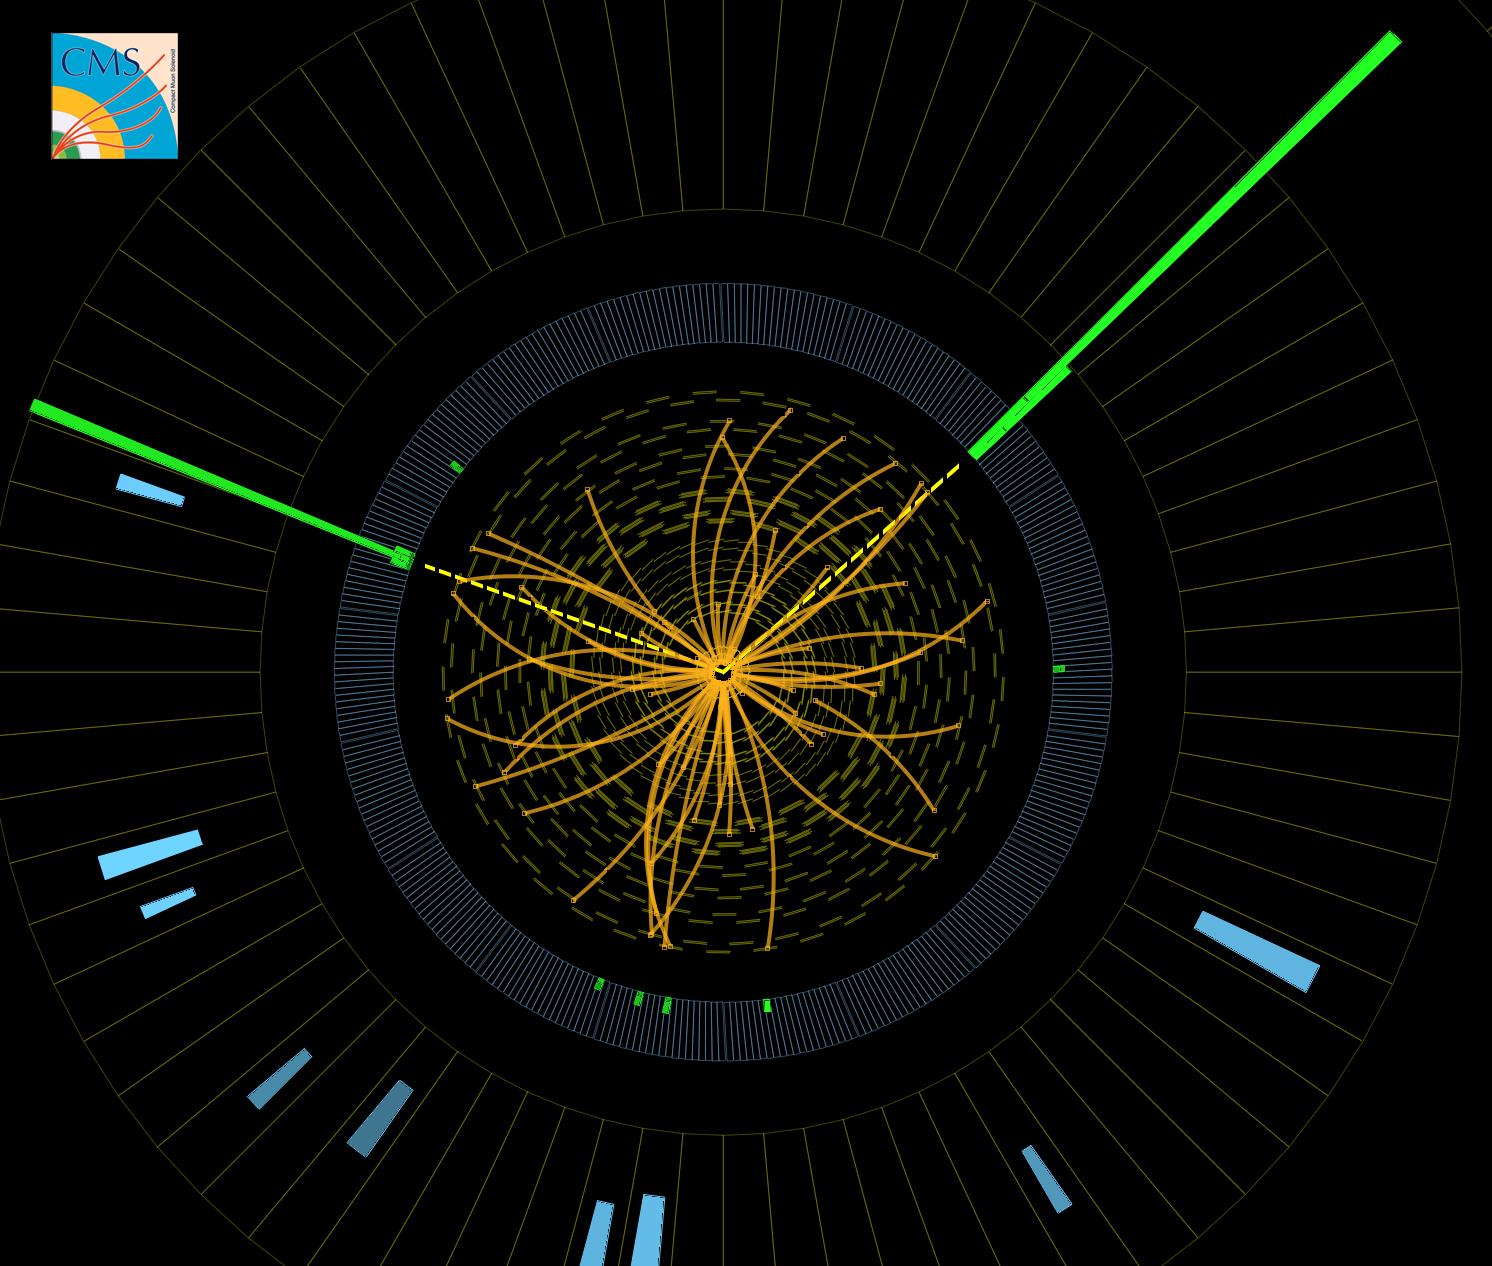
\includegraphics[width=0.48\textwidth]{../plots/cms_event_display.png}
\hfill
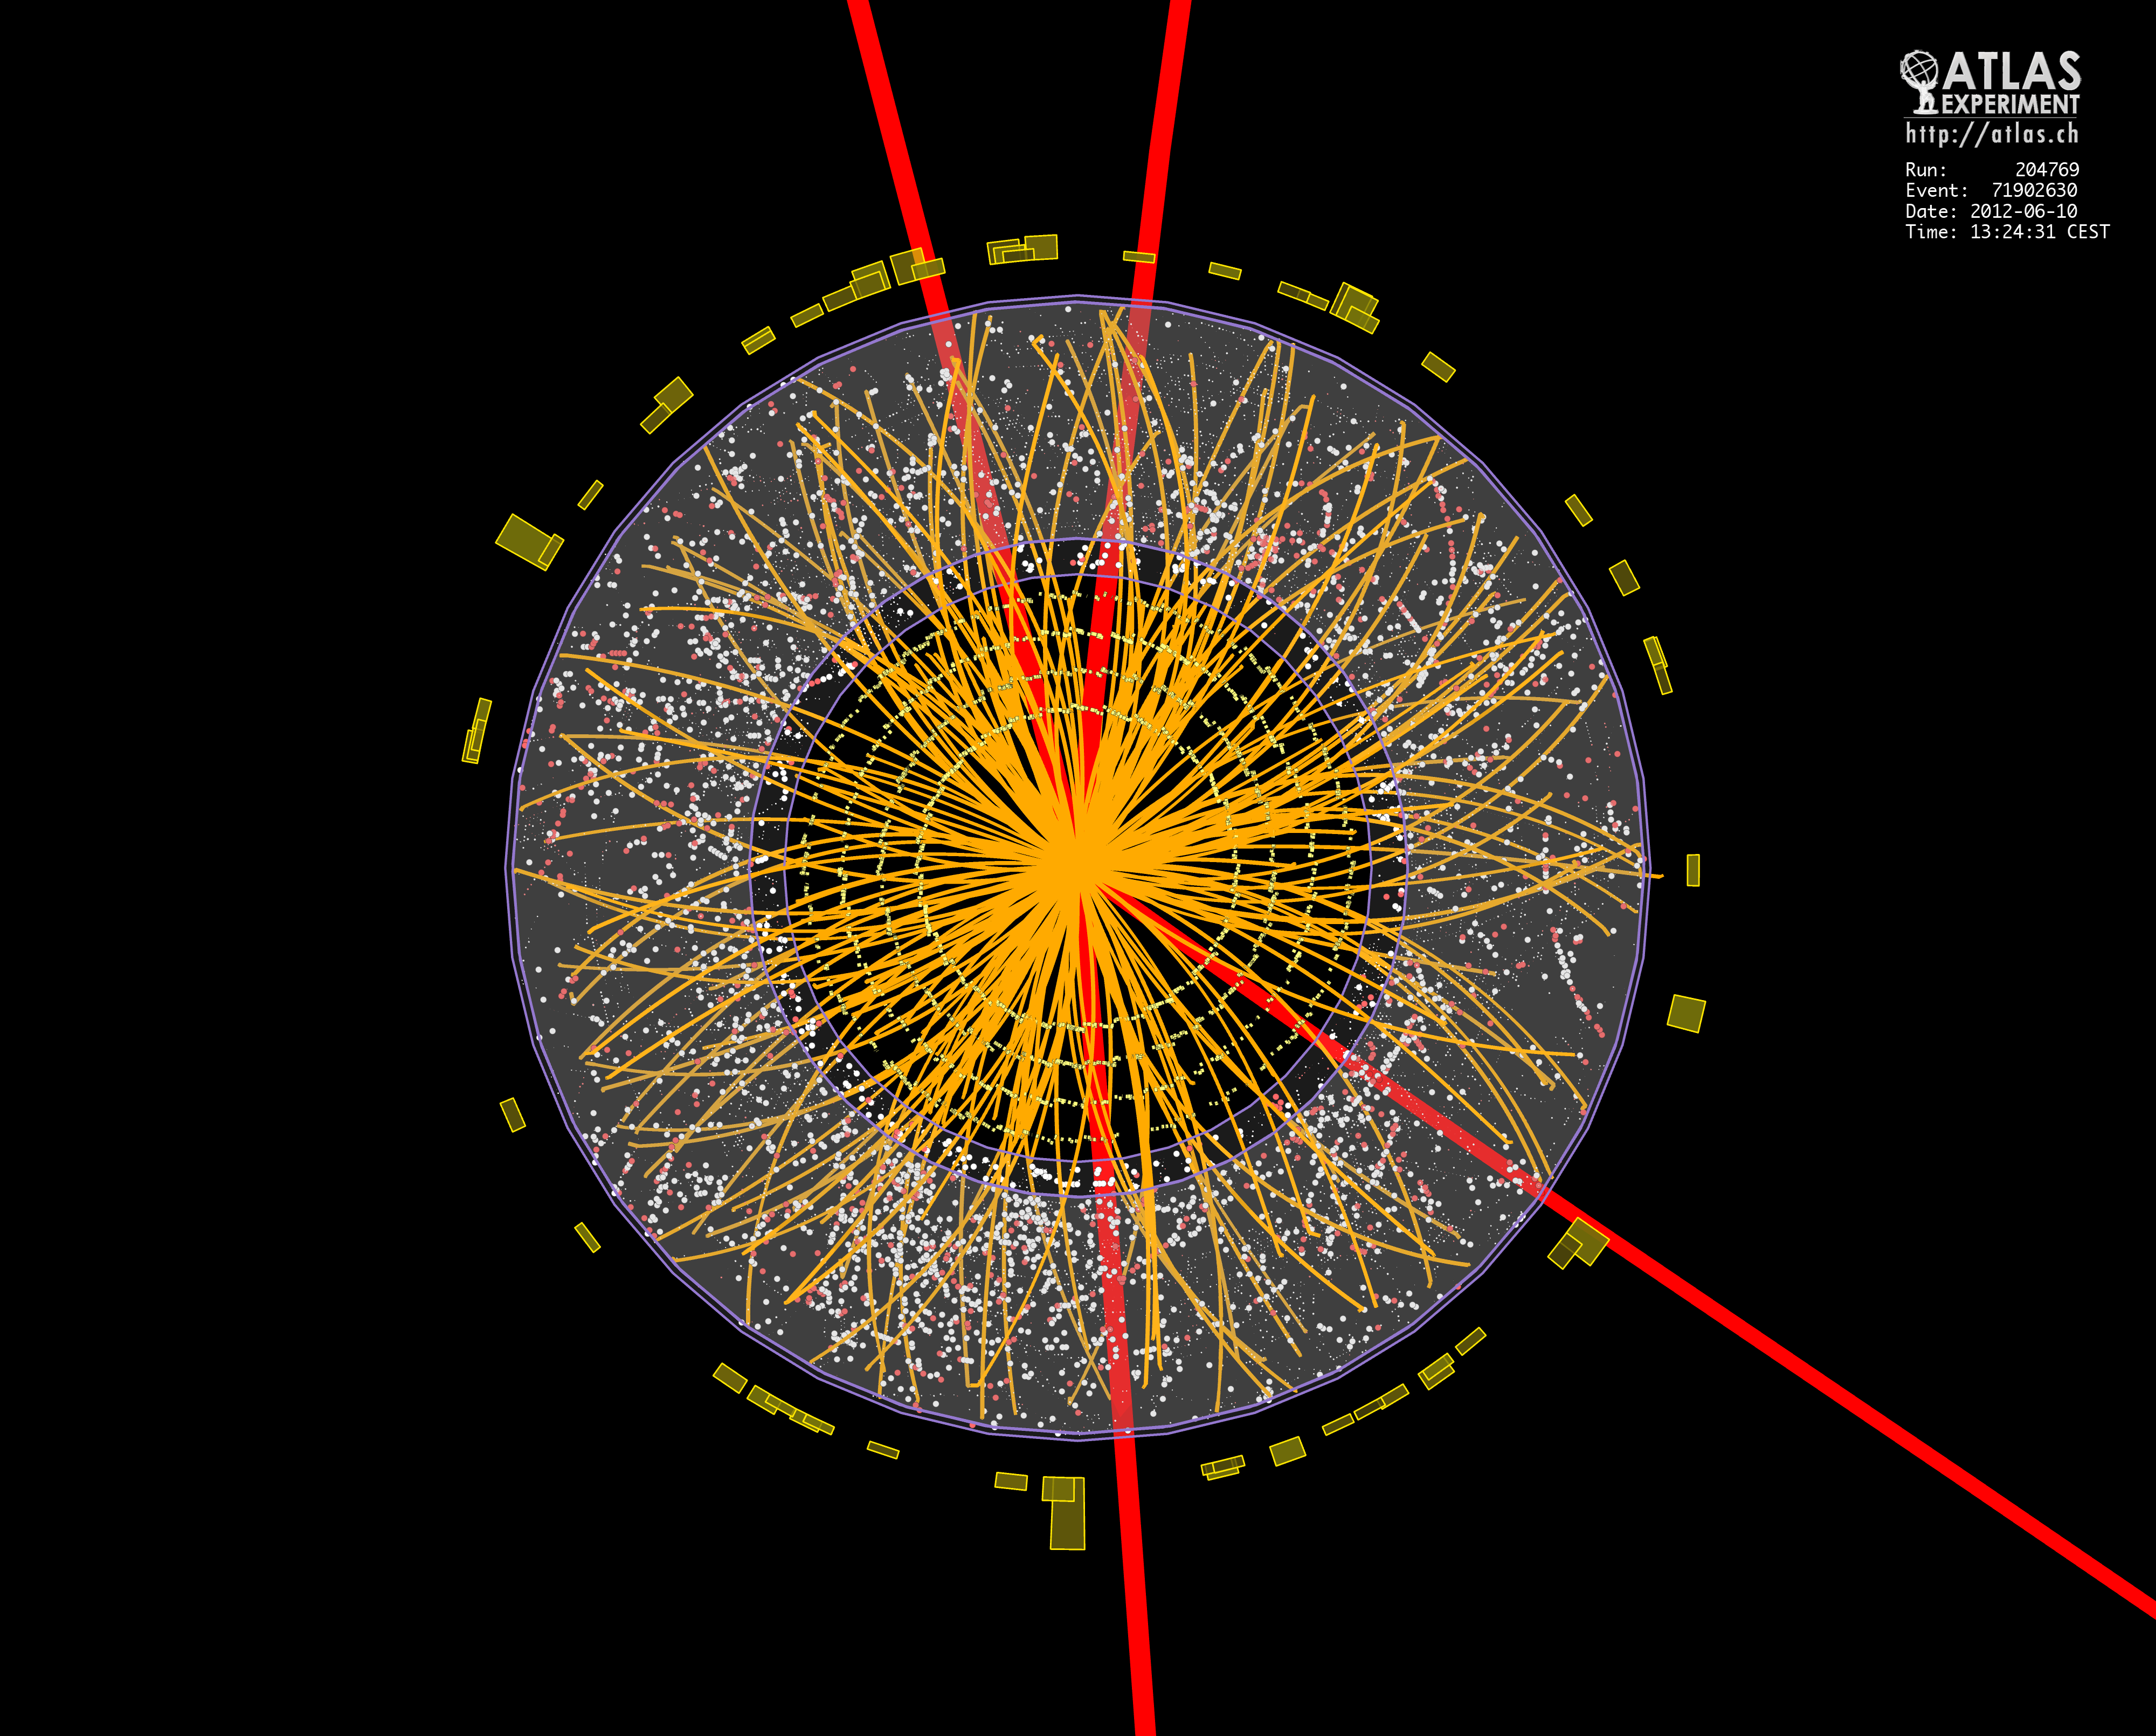
\includegraphics[width=0.48\textwidth]{../plots/atlas_event_display.png}
\caption[Higgs boson discovery CMS.]{Higgs boson decay event displays in the two golden channels $\PH \rightarrow \Pgamma \Pgamma$ (left: \CMS) and $\PH \rightarrow \PZ \PZ \rightarrow 4\Plepton$ (right: \ATLAS).}
\label{figure_higgs_discovery_eventdisplay}
\end{figure}

In the left event display~\ref{figure_higgs_discovery_eventdisplay} one can clearly see entries in the electromagnetic calorimeter (ECAL) but not tracks (hinted with the dotted line).
It is the signature of two photons, which interact electromagnetically (entries in ECAL) and have no electrically charge (no tracks). From the event display it is not
possible to reconstruct the invariant mass, therefore it provides only the signatures in the detector for a Higgs boson candidate.

The right event display~\ref{figure_higgs_discovery_eventdisplay} shows four leptons in the detector. Furthermore one can specify them as muons, since they
penetrate the whole detector complex. Unlike photons muons have an electrically charge and therefore leave a track in the inner tracker system of the detector.
This event display also can only show a Higgs boson candidate, since the essential invariant mass information is missing.

In order to prove the observation of the Higgs boson statistical methods are needed. In fact it is a common strategy to perform
hypothesis testing for the theory with and without the Higgs boson. They allow to quantify the compatability between the SM with a Higgs boson and
without a Higgs boson at a certain confidence level (usually chosen to be $95\%$). Figure~\ref{figure_higgs_discovery_limit} (left) shows the limit for a SM Higgs hypothesis as a function
of different mass hypothesis. A clear excess of the data can be observed in the mass interval of $120$ GeV to $130$ GeV. This means that one can not exclude a Higgs boson with $120 < m_H <130$ GeV
with the measured data of Run 1 from the SM.

\begin{figure}[h]
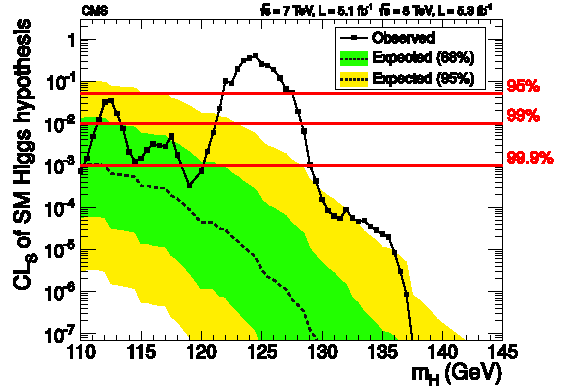
\includegraphics[width=0.48\textwidth]{../plots/higgs_combined_cls.pdf}
\hfill
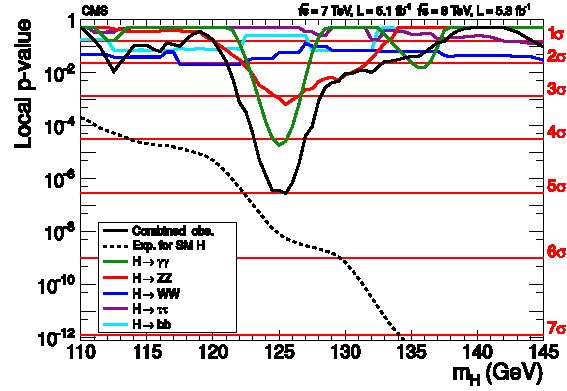
\includegraphics[width=0.48\textwidth]{../plots/higgs_p_value.pdf}
\caption[Higgs boson discovery CMS limit.]{Expected and observed limit (left) and local p-value (right) as a function of different mass hypothesis ~\cite{HiggsDiscovery_CMS}.}
\label{figure_higgs_discovery_limit}
\end{figure}

Additionally it is possible to quantify the statistical significance of the measured excess.
The local p-value is calculated as a function of the Higgs boson mass. From figure~\ref{figure_higgs_discovery_limit} (right) it is clear
that the combined observed limit shows an excess of $5.0\sigma$, making it a discovery. At the same time the best fit result for the Higgs mass
can be extracted. It is measured to be:
\begin{itemize}
  \item CMS: $m_H= 125.3 \pm 0.4 \,\text{(stat)} \pm 0.5 \,\text{(sys)}\, \text{GeV}$~\cite{HiggsDiscovery_CMS}
  \item ATLAS: $m_H= 126.0 \pm 0.4 \, \text{(stat)} \pm 0.4 \, \text{(sys)}\, \text{GeV}$~\cite{HiggsDiscovery_ATLAS}
\end{itemize}


\begin{figure}[h]
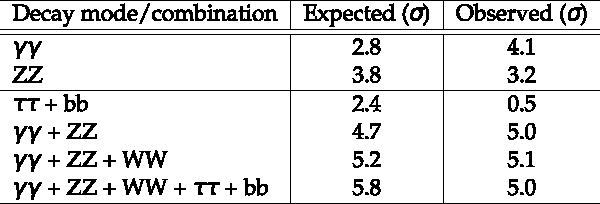
\includegraphics[width=0.75\textwidth]{../plots/higgs_pvalue_table.pdf}
\caption[Higgs boson discovery CMS limit.]{Table of expected and observed statistical significances for different decay channel~\cite{HiggsDiscovery_CMS}.}
\label{figure_higgs_discovery_pvalue}
\end{figure}

The expected and observed significance for all analysed decay channels is depicted in table~\ref{figure_higgs_discovery_pvalue}. It can be seen that
including the $\PH \rightarrow \Ptau \Ptau$ and $\PH \rightarrow \Pbottom \APbottom$ the observed significance drops again. This was due to a bad statistical
fluctuation in the measurement by \CMS.


\section{Golden Channel: $\PH \rightarrow \PZ \PZ \rightarrow 4\Plepton$ \label{golden_channel}}

Although branching fraction of the $\PH \rightarrow \PZ \PZ \rightarrow 4\Plepton$ is quite small ($\approx2.6\%$) it provides a very high
mass resolution and a straight forward reconstruction of the Higgs boson. The basic analysis strategy is to start with the four leptons, which
are measured in the detector, and then reconstruct the $\PZ$ bosons. Afterwards the two $\PZ$ bosons can be combined to the Higgs boson.

As aforementioned one can only start this analysis by selecting four leptons. The possible combinations in this case are: $4\Pe$, $4\Pmu$ or $2\Pe2\Pmu$.
The tau leptons are neglected here, since their reconstruction efficiency is quite small in comparision to muons and electrons. The selection of the
four leptons is done by introducing basic requirements. These cuts reject pile-up events (remnants from pp collisions), which one can see in the event displays from figure~\ref{figure_higgs_discovery_eventdisplay}
as the yellow tracks.

Afterwards it is necessary to reconstruct $\PZ$ boson candidates from the lepton selection. Two opposite sign same flavour leptons are combined. Their resulting invariant
mass has to pass a mass window cut of $12 < m_{ll} < 120$ GeV. One of the combination is required to have the mass of the $\PZ$ mass, since one $\PZ$ boson is produced on-shell: $m_{ll}\approx m_{\PZ}$. The remaining
two leptons are combined to a off-shell $\PZ^*$ boson. For each event one can now combine the invariant mass of the four leptons of the $\PZ\PZ^*$
selection in order to reconstruct the Higgs boson.

After the introduced event selection, the analysis has some remaining irreducible backgrounds. First of all there is the non-resonant $\PZ\PZ$ and $\PZ\Pgamma^*$ process.
From figure~\ref{figure_higgs_background} it is obvious that they represent the main background of this analysis. The other irreducible background are merged into one background class, the so-called $\PZ + \mathrm{X}$ process.
This process is the combination of the following 5 background contributions: $\PZ+$jets, $\Ptop\APtop+$jets, $\PZ\Pgamma+$jets,
$\PW\PW+$jets and $\PW\PZ+$jets. These processes do not leave four leptons in the detector, but instead the jets are misidentified as leptons by the reconstruction requirements.
The rate of this is rather small, but non-negligible.

\begin{figure}[h!]
\centering
\begin{tikzpicture}[line width=1.5pt, scale=1.2]
\draw[step=0.5cm, very thin, transparent] (0cm,0cm) grid (4cm,2cm);

\draw[fermionbar] (0cm,0cm) -- (1.25cm,1cm);
\node at (0cm-0.2cm,0cm) {$\overline{q}$};

\draw[fermion] (0cm,2cm) -- (1.25cm,1cm);
\node at (0cm-0.2cm,2cm) {$q$};

\draw[fermionbar] (2.75cm,1cm) -- (4cm,2cm);
\node at (4cm+0.3cm,2cm) {$l^+$};

\draw[vector] (2.75cm,1cm) -- node[below]{$\textcolor{color1}{Z}$} (1.25cm,1cm);

\draw[fermion] (2.75cm,1cm) -- (4cm,0cm);
\node at (4cm+0.4cm,0cm) {$l^-$};

\draw[vector] (3.05cm,1.25cm) -- (4cm,1.25cm);
\node at (4cm+0.4cm,1.25cm) {$\textcolor{color1}{Z/\gamma^*}$};
\end{tikzpicture}

\caption{Feynman diagram of the non-resonant background $\PZ\PZ$ and $\PZ\Pgamma^*$ in the $\PH \rightarrow \PZ \PZ \rightarrow 4\Plepton$ analysis.}
\label{figure_higgs_background}
\end{figure}

This analysis was done again with Run 2 data. The Higgs boson was rediscovered, which marks a hugh success. Figure~\ref{figure_higgs_rediscovery_atlas} shows the rediscovery with data of $\luminosity=36.1\fbinv$ taken in year
2016. A brand new (still on-going) analysis is currently at pre-approval. Therefore the signal region is still blinded in figure~\ref{figure_higgs_rediscovery_cms}. Both plots show clearly an observed (expected) excess in data measured
by ATLAS (CMS). Because of a higher integrated luminosity, the increase in center-of-mass energy from Run 1 to Run 2 and the improved analysis strategy, the excess in the four-lepton mass spectrum is larger than before.

\begin{figure}[h]
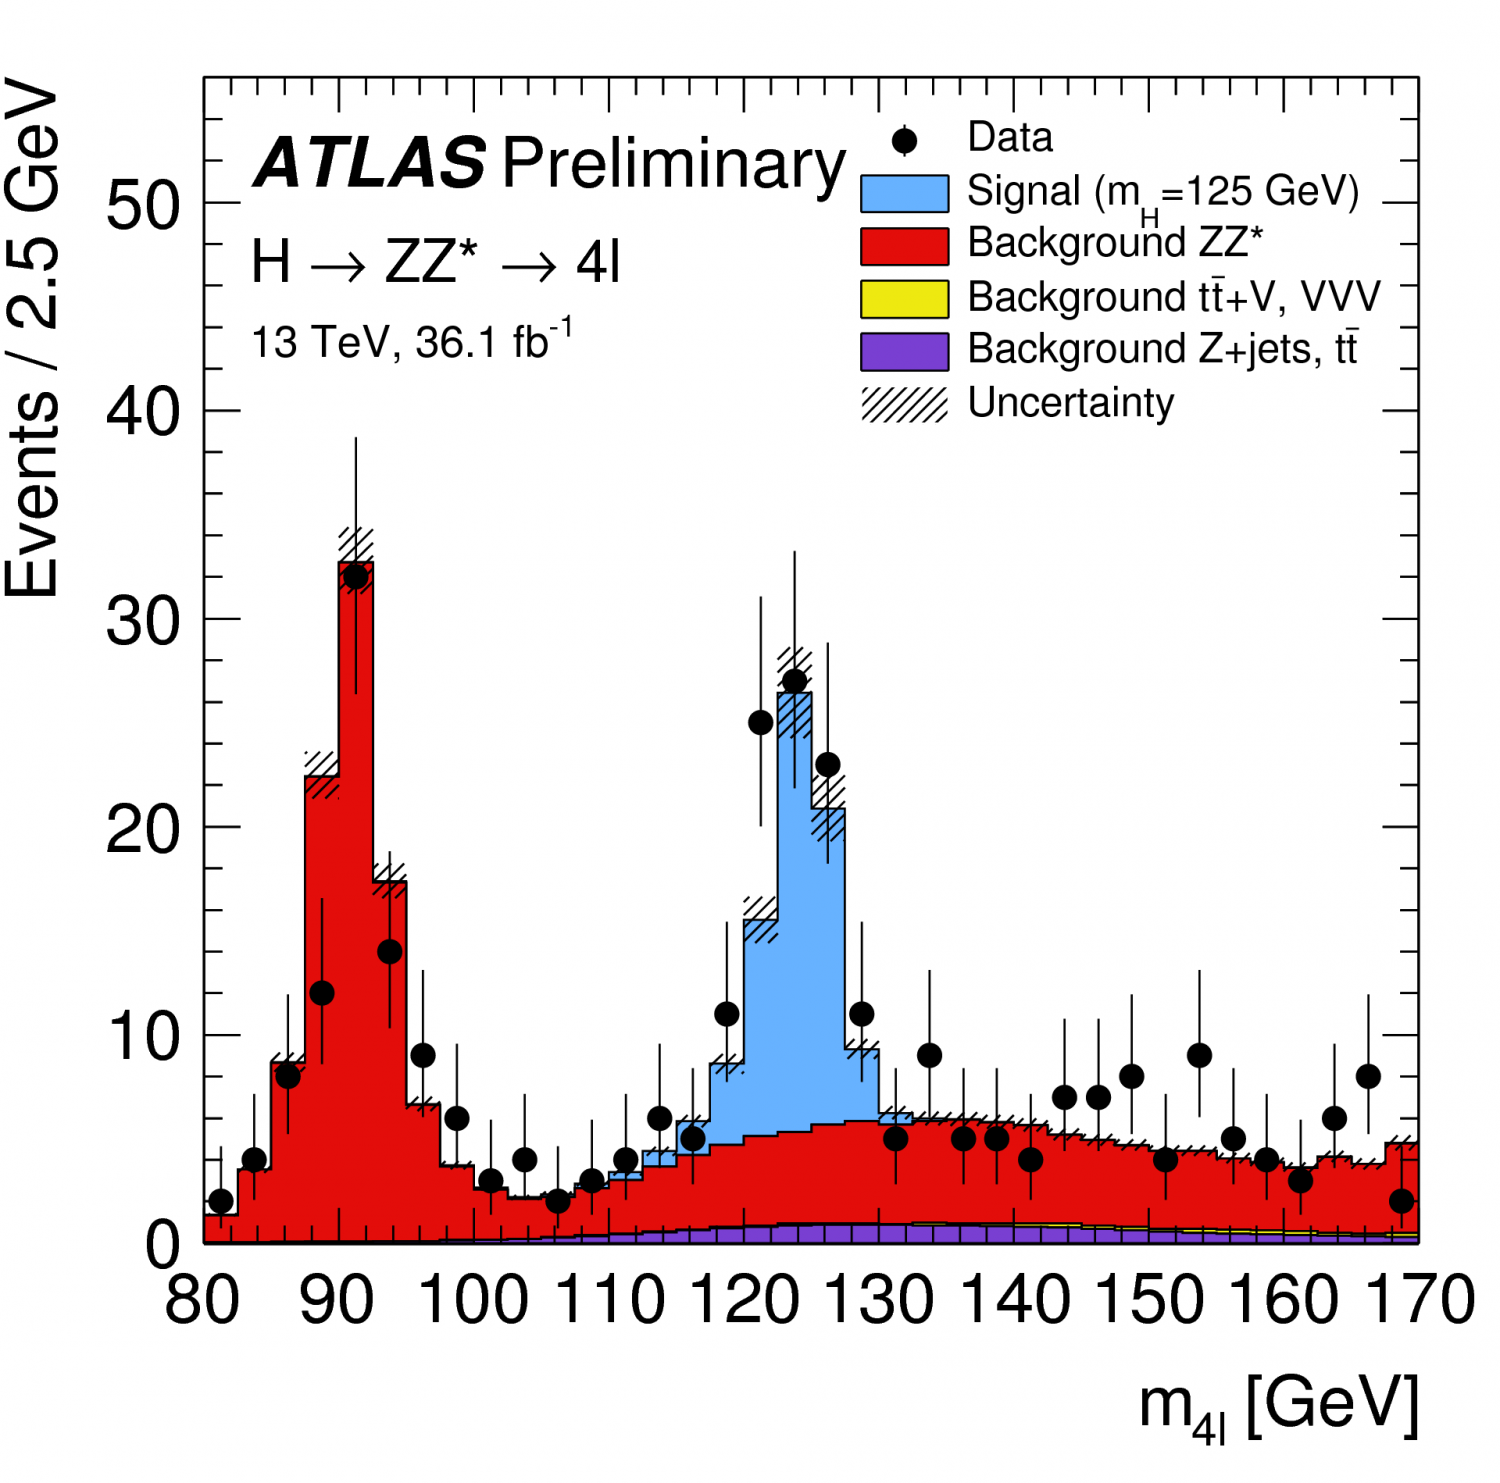
\includegraphics[width=0.48\textwidth]{../plots/2016_goldenchannel.png}
\caption[Higgs boson rediscovery.]{Higgs rediscovery in golden channel with 2016 data by ATLAS~\cite{HiggsReDiscovery_ATLAS}.}
\label{figure_higgs_rediscovery_atlas}
\end{figure}

\begin{figure}[h]
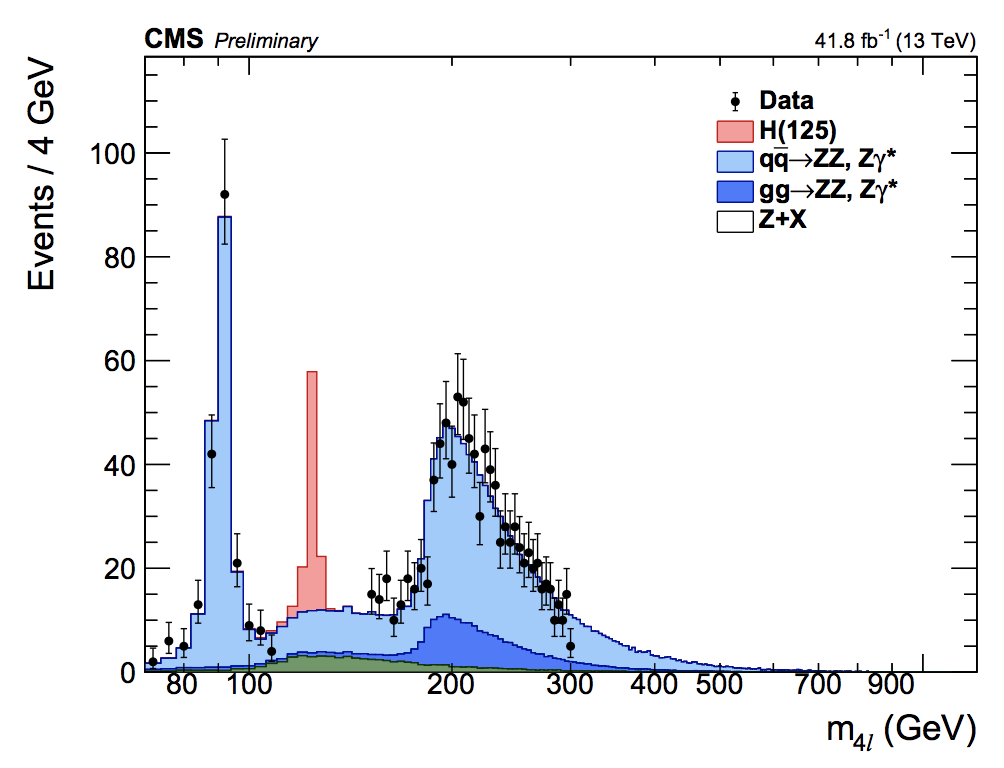
\includegraphics[width=0.48\textwidth]{../plots/2017_goldenchannel}
\caption[Higgs boson rediscovery.]{Brand new analysis with 2017 data by CMS~\cite{HiggsReDiscovery_CMS} (right, still blinded)}
\label{figure_higgs_rediscovery_cms}
\end{figure}

\section{Recent $\PH \rightarrow \Ptau \Ptau$ Discovery \label{HTT}}

In Run 1 the search for the SM Higgs boson decaying into a pair of tau leptons suffered from bad statistical fluctuations. Additionally this measurement
is very challenging, since the reconstruction efficiency of tau leptons is rather bad in comparison to electrons and muons. Also this search has to deal with
the QCD background, which is very hard to predict and badly modelled by Monte Carlo (MC) simulations.

Recently the decay of the SM Higgs boson into a pair of tau leptons could be observed by \CMS. One of the most important approach in this analysis is to predict the QCD background from an exclusive
region in data (not from MC). Using the ABCD method one is able to construct control regions for this background and therefore constrain
the systematic uncertainty of the QCD cross-section. Additionally the analysis is splitted into different categories in order to enhance the sensitivity: 0-jet, VBF and boosted category.
Figure~\ref{figure_higgs_discovery_HTT} shows the two discovery plots of the
$\PH \rightarrow \Ptau \Ptau$ analysis. One can clearly see and excess in data in the invariant di-tau mass spectrum. This is especially visible in the "integrated" figure, where
data minus background is shown. The statistical significance of the analysis is measured to be $5.9\sigma$, making it a discovery. The best fit value for the SM Higgs boson
signal strength is $\mu = 1.09_{-0.26}^{+0.27}$ at a Higgs boson mass of $m_{H} = 125.09$ GeV.

\begin{figure}[h]
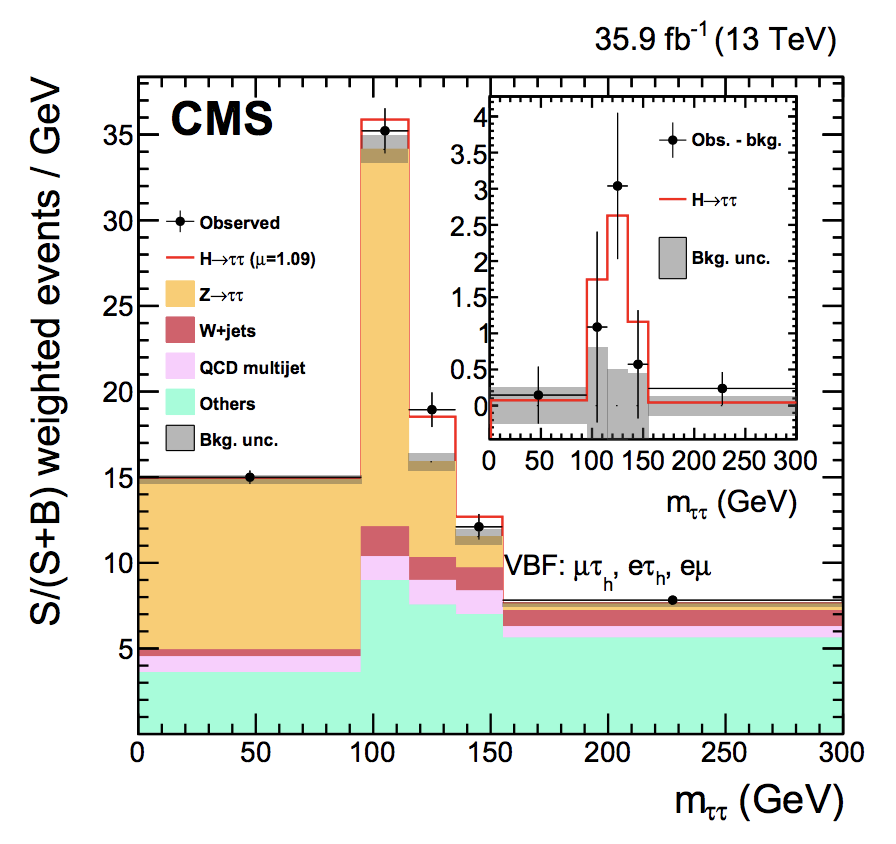
\includegraphics[width=0.48\textwidth]{../plots/higgstautau_otherchannel.png}
\hfill
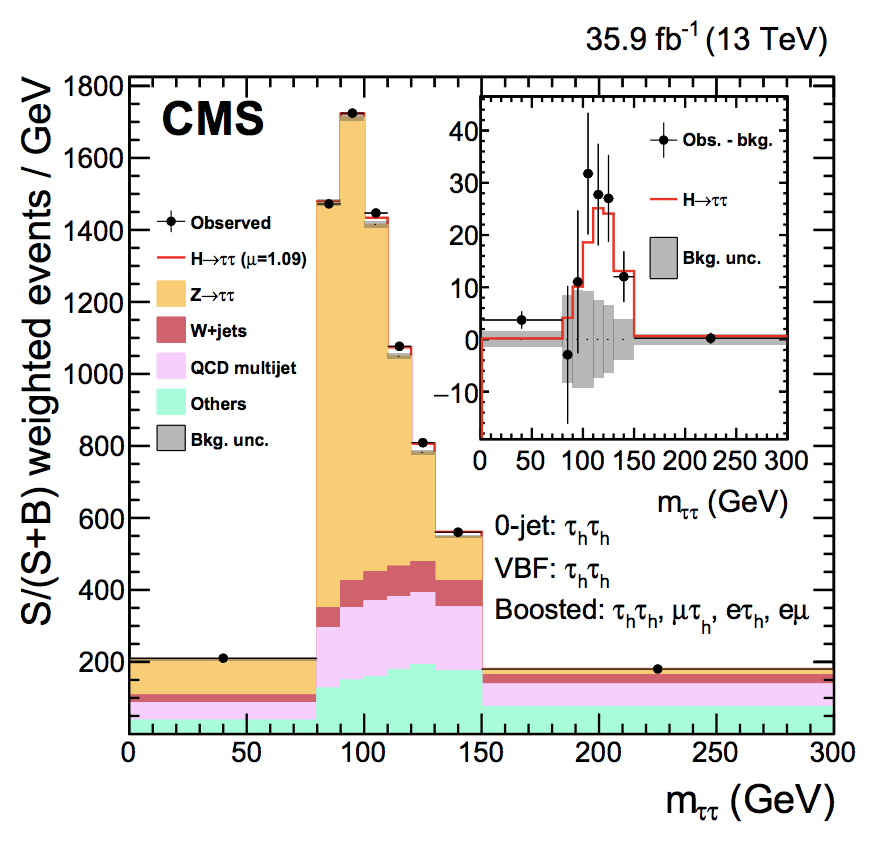
\includegraphics[width=0.48\textwidth]{../plots/higgstautau.png}
\caption[Higgs boson discovery $\PH \rightarrow \Ptau \Ptau$.]{Discovery plots of a SM Higgs boson decaying into a pair of tau leptons. Left: Semi-leptonic decay channels. Right: Full-hadronic decaychannel.~\cite{HTT_discovery}.}
\label{figure_higgs_discovery_HTT}
\end{figure}
